\documentclass{beamer}

%%% Fichier de préambule avec toutes les définitions communes aux trois diaporamas

% Packages
\usepackage[utf8]{inputenc}  % Encodage : UTF-8
\usepackage[T1]{fontenc}     % Caractères français

\usepackage[french]{babel}   % Langue française

\usepackage{amsmath}         % Maths améliorées
\usepackage{amssymb}         % Symboles mathématiques
\usepackage{amsfonts}        % Polices mathématiques
\usepackage{graphicx}        % Inclusion d'images (PNG, GIF, PDF)
\usepackage{array}           % Tableaux améliorés
\usepackage[normalem]{ulem}  % Styles barré et souligné
\usepackage{listings, multicol, xcolor} % Listings (code source)
\usepackage{lmodern}         % Police d'écriture
\usepackage{url, hyperref}   % Liens hypertexte

\usepackage{tikz}            % TikZ : figures avancées
\usepackage{circuitikz}      % Circuits électriques en TikZ
% Diverses bibliothèques pour TikZ
\usetikzlibrary{chains, calc, decorations.pathmorphing, fadings, shadings, arrows, decorations.pathreplacing, shapes} 



% Commande \meta pour les listings
\newcommand{\meta}[1]{\ensuremath\langle\itshape#1\ensuremath\rangle}

% Paramètres des listings
\lstset{
upquote=false,
columns=flexible,
basicstyle=\ttfamily\scriptsize,
language={[LaTeX]TeX},
identifiersstyle=\color{green},
emphstyle=\color{blue},
keywordstyle=\color{blue},
directivestyle=\color{blue},
commentstyle=\color{gray},
    inputencoding=utf8,
literate={eacute}{\'e}1,    % Permet de faire des accents dans un listing avec £\'e£, £\`e£, £\`a£
    {eagrave}{\`e}1,
    {aagrave}{\`a}1,
    escapechar={£},
    moretexcs={meta},
morekeywords={              % Mots-clefs supplémentaires
  part,chapter,subsection,subsubsection,
  frontmatter,mainmatter,backmatter,
  tableofcontents,listoffigures,listoftables,titlepage,
  includegraphics,includepdf,
  dddot,ddddot,
  frametitle,framesubtitle,
  pause,only,uncover,
  usetheme,usecolortheme,
  institute,maketitle,
  usetikzlibrary,
  node,path,
  commande
}
}



% Thème Beamer
\usetheme{CambridgeUS}



% Auteurs et licence
\author[Folschette, Jubien, Tanguy]{Maxime \textsc{Folschette\up{1} } \and Anthony \textsc{Jubien\up{2}} \and Julien \textsc{Tanguy\up{3}} \\ 
{\scriptsize  \up{1} IRCCyN équipe MeForBio \\
\up{2} IRCCyN équipe Robotique et ONERA Toulouse \\
\up{3} IRCCyN équipe Systèmes Temps Réels \\
maxime.folschette, anthony.jubien, julien.tanguy @irccyn.ec-nantes.fr} }
\institute[AED]{Association des Étudiants en Doctorat de l'ECN (AED)  \\ 
Document sous licence Creative Commons BY 3.0 FR \\
http://creativecommons.org/licenses/by/3.0/fr/}



% Suppression des icônes de navigation
\setbeamertemplate{navigation symbols}{}

% Sommaire au début de chaque partie
\AtBeginPart{%
    \frame{\partpage}

    \begin{frame}
        \frametitle{Plan}
        \tableofcontents
    \end{frame}
}


\title{Séminaire \LaTeX, séance 1: prise en main}
\date{jeudi 21 février 2013}

\begin{document}

%%%%%%%%% SLIDE %%%%%%%%%%%%%%%%%%

\begin{frame}
    \titlepage
\end{frame}

%%%%%%%%% SLIDE %%%%%%%%%%%%%%%%%%

\begin{frame}{Points abordés durant la séance 1:}
    \begin{itemize}
            \item présentation théorique de \LaTeX,
            \item installation des outils nécessaires sur les machines de chacun,
            \item commandes basiques amenant à la création de documents simples. 
        \end{itemize}
\end{frame}

%%%%%%%%%%%%%%%%%%%%%%%%%%%%%%
%%%%%%%%%%%% PART %%%%%%%%%%%%%%%
%%%%%%%%%%%%%%%%%%%%%%%%%%%%%%

%\part{Introduction}

%%%%%%%%%%%%%%%%%%%%%%%%%%%%%%
%%%%%%%%%%% SECTION %%%%%%%%%%%%%%
%%%%%%%%%%%%%%%%%%%%%%%%%%%%%%

\section{Présentation de \LaTeX} 

%%%%%%%%% SLIDE %%%%%%%%%%%%%%%%%%

\begin{frame}{Introduction}
    \begin{block}{Qu'est que \LaTeX?}
        \begin{itemize}
            \item un logiciel de composition typographique
            \item permet la production de documents scientifiques de grande qualité avec une grande souplesse
            \item polyvalent: thèses, rapports, publications, livres, lettres, cv, présentations, etc\dots
        \end{itemize}
    \end{block}
    \begin{block}{Qu'est que n'est pas \LaTeX?}
        \begin{itemize}
            \item un traitement de texte
            \item un outil facile à prendre en main\footnote{D'où ce cours \dots}
        \end{itemize}
    \end{block}
\end{frame}

%%%%%%%%% SLIDE %%%%%%%%%%%%%%%%%%

\begin{frame}{Comparaison avec Microsoft Word/ OpenOffice Writer}
    \begin{block}{Microsoft Word / OpenOffice Writer}
        \begin{itemize}
 	\item ce qui est affiché à l'écran est le document imprimé
            \item pas ou peu d'apprentissage
            \item interface graphique
            \item difficulté pour changer la mise en forme du document
            \item incompatibilité entre certaines versions du logiciel
            \item gestion de la bibliographie plus ou moins hasardeuse
     \item typographie des équations mathématiques hasardeuse
        \end{itemize}
    \end{block}
\end{frame}

%%%%%%%%% SLIDE %%%%%%%%%%%%%%%%%%

\begin{frame}{Comparaison avec Microsoft Word/ OpenOffice Writer}
    \begin{block}{\LaTeX}
        \begin{itemize}
            \item sépare en deux phases la forme du contenu
            \item apprentissage initial important
            \item gère facilement des gros documents
            \item compatibilité permanente
            \item gestion des équations mathématiques et de la bibliographie exemplaire
	 \item multi-plateformes
        \end{itemize}
    \end{block}
\end{frame}

%%%%%%%%% SLIDE %%%%%%%%%%%%%%%%%%

\begin{frame}{Comparaison visuelle}

\begin{figure}
\centering
  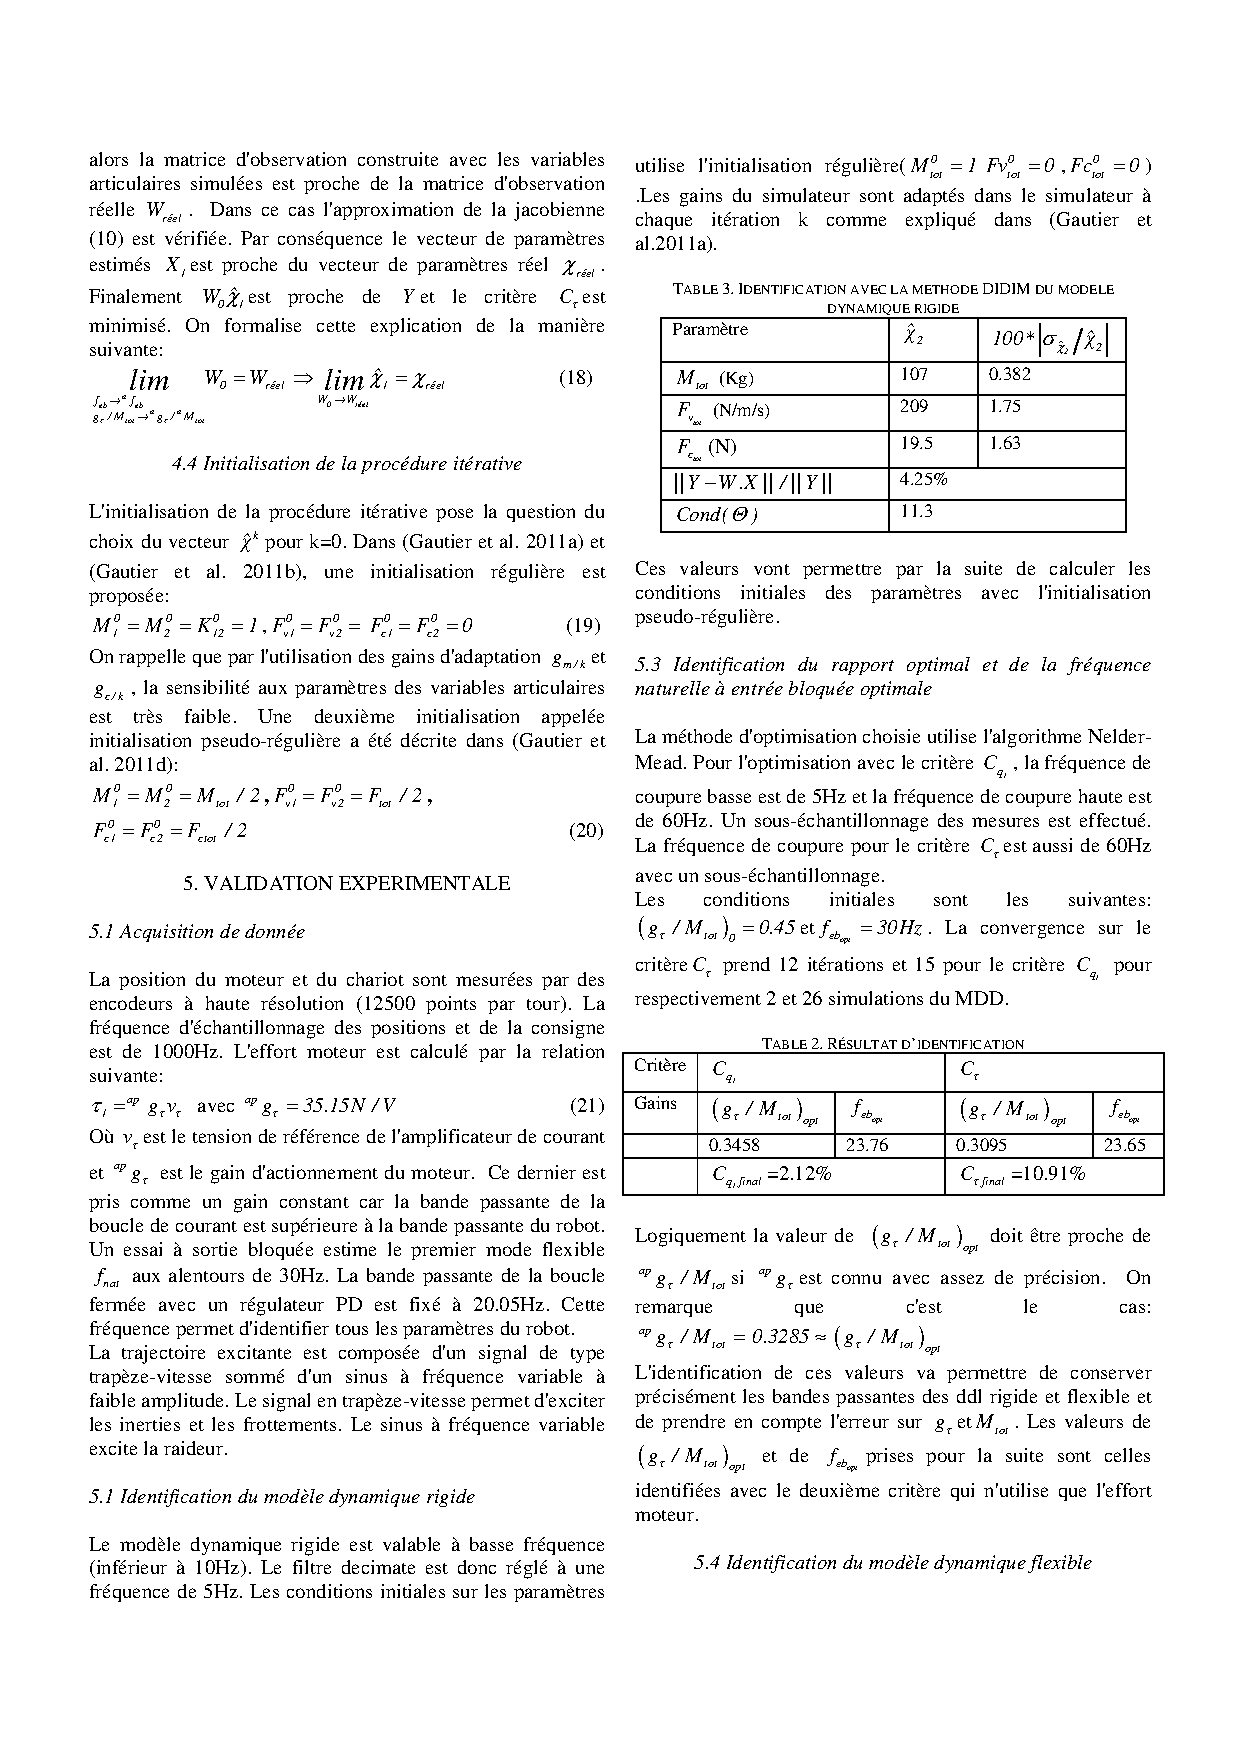
\includegraphics[width= 10cm, trim = 0cm 22cm 0cm 0cm, clip]{img/cifa_word} 
%\end{figure}

%\begin{figure}
%\centering
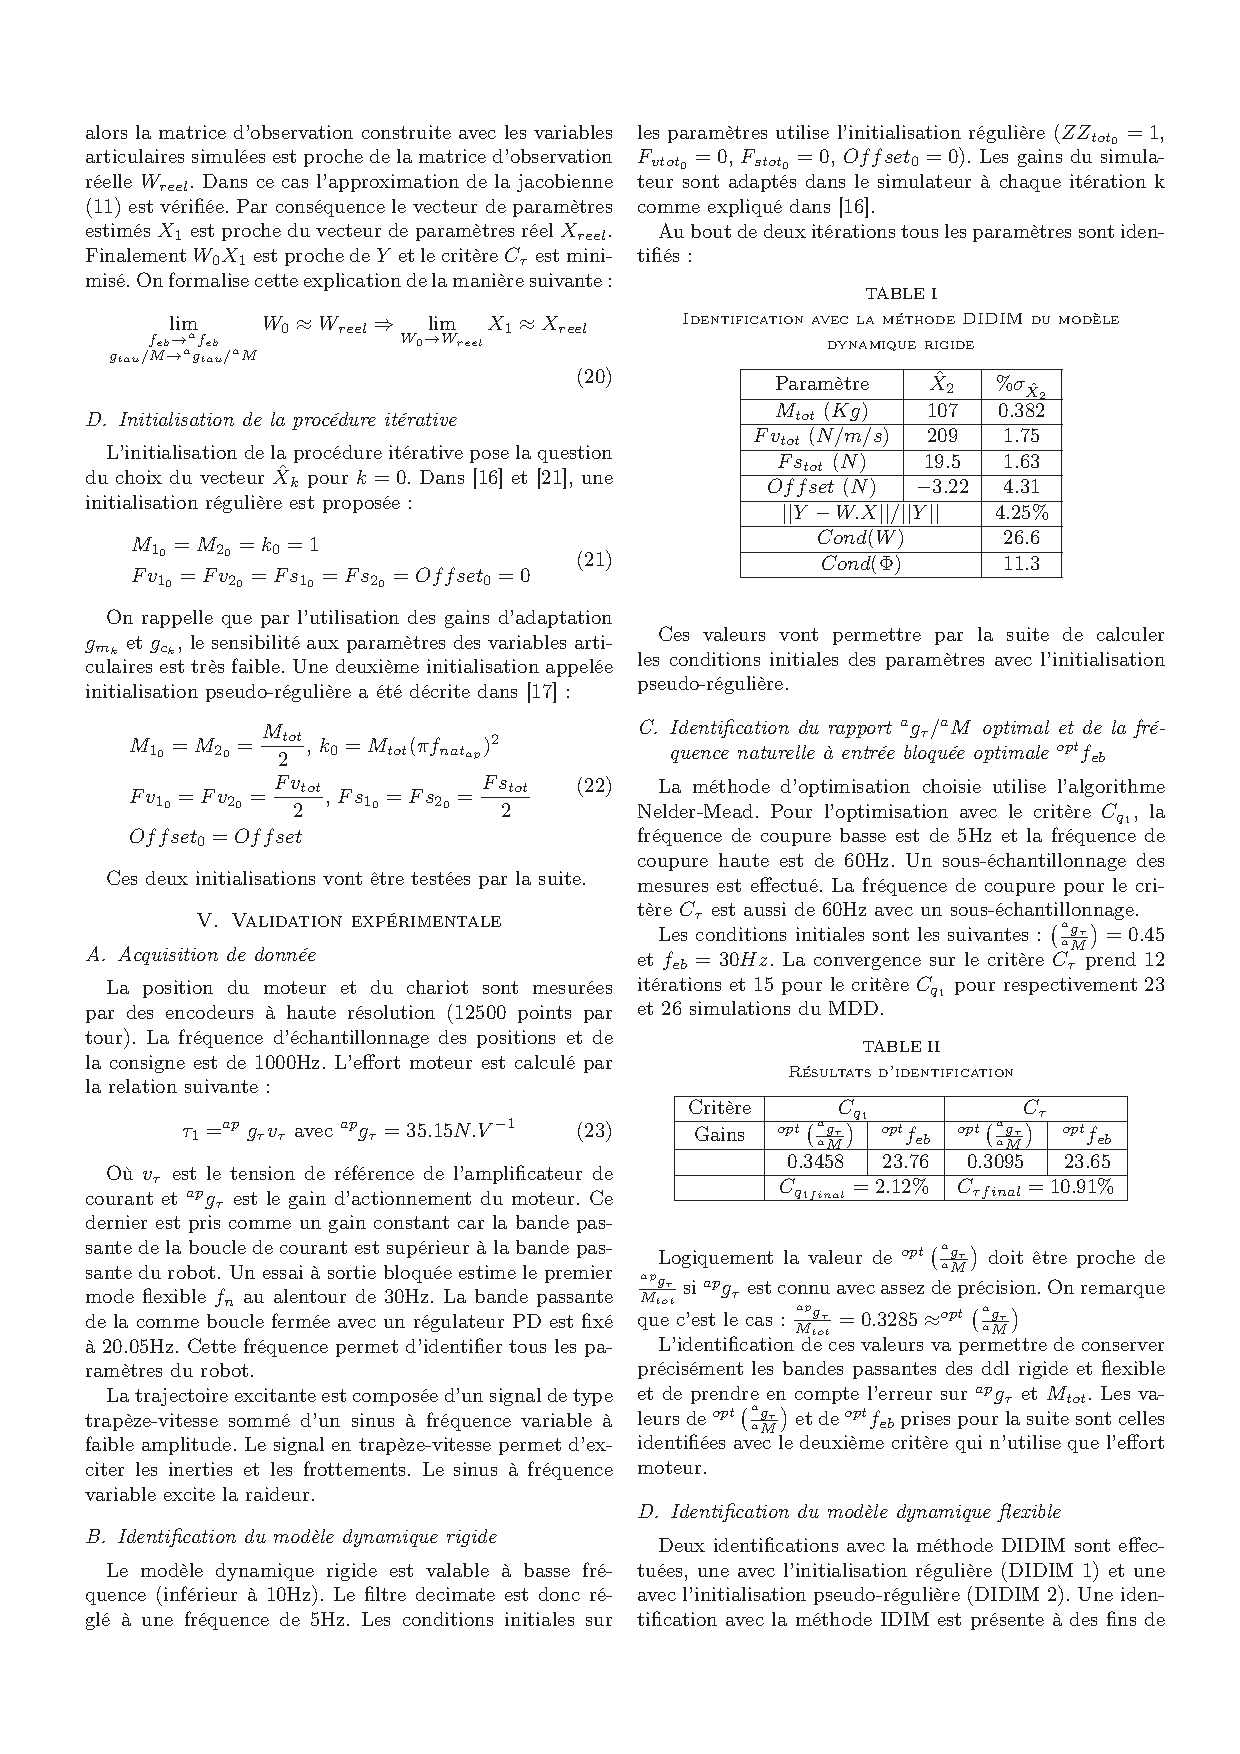
\includegraphics[width=10 cm, trim = 0cm 21cm 0cm 0cm, clip]{img/cifa_latex}
\end{figure}

\end{frame}



%%%%%%%%% SLIDE %%%%%%%%%%%%%%%%%%

\begin{frame}{Principes de base}
    \begin{itemize}
        \item un peu le même principe que le langage HTML
        \item cycle de type édition-compilation
        \item au départ: document source (.tex)
        \item à l'arrivée: document de type pdf (.pdf)
    \end{itemize}
\end{frame}

\begin{frame}{Un peu de vocabulaire}
    \begin{description}
        \item[Distribution \LaTeX :] ensemble de programmes et paquets permettant de compiler un document tex
        \item[Éditeur \LaTeX       :] éditeur facilitant l'écriture de documents \LaTeX: jEdit, Notepad++, TeXnicCenter, TeXmaker, etc.
    \end{description}
\end{frame}


%%%%%%%%% SLIDE %%%%%%%%%%%%%%%%%%

\section{Installation} 

\begin{frame}{Distribution \LaTeX}
    \begin{block}{Windows 
\includegraphics[width=0.6 cm]{img/logo_win7} }
        \begin{description}
            \item[Distribution] MiK\TeX{} \url{http://miktex.org}
            \item[Éditeur] Texmaker \url{http://www.xm1math.net/texmaker/index_fr.html}
        \end{description}
    \end{block}
    \begin{block}{Mac OS 
\includegraphics[width=0.6 cm]{img/logo_apple} }
        Mac\TeX{} \url{http://tug.org/mactex} (distribution et éditeur)
    \end{block}
    \begin{block}{Linux 
\includegraphics[width=0.6 cm]{img/logo_linux}}
        \begin{description}
            \item[Distribution] TeXlive (installer les paquets \texttt{texlive}, \texttt{cm-super})
            \item[Éditeur] Kile (paquet \texttt{kile})
        \end{description}
    \end{block}
\end{frame}

%%%%%%%%% SLIDE %%%%%%%%%%%%%%%%%%

\begin{frame}{Téléchargement}

\begin{figure}
\centering
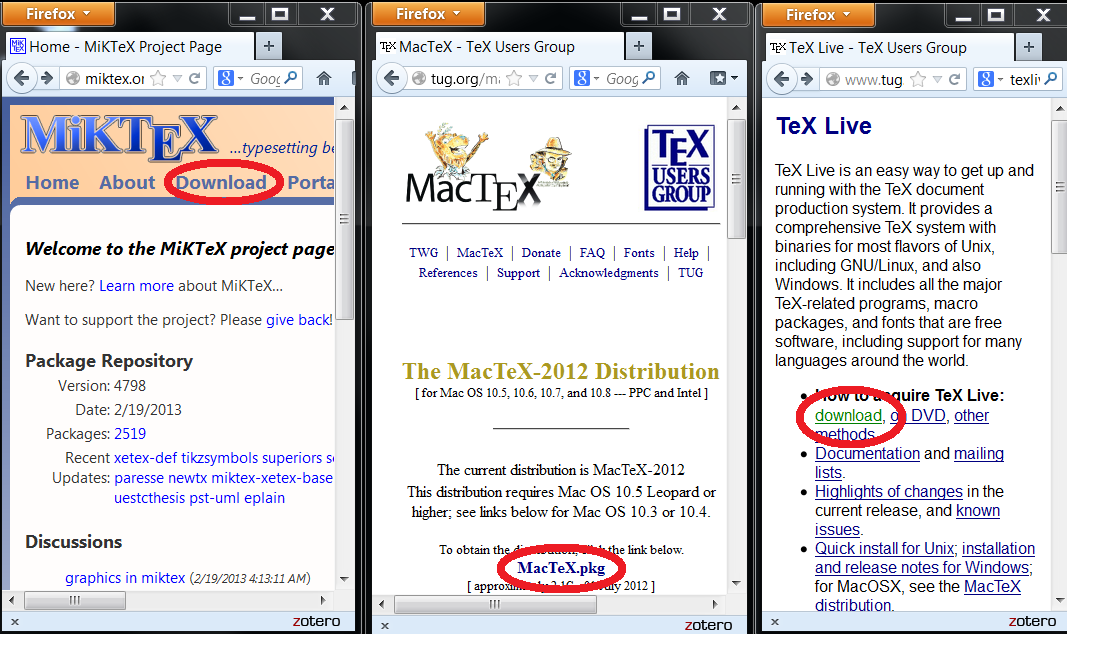
\includegraphics[width=11cm]{img/fenetre_moz_log}
\end{figure}

\end{frame}

%%%%%%%%% SLIDE %%%%%%%%%%%%%%%%%%

\begin{frame}{MikTeX (Windows)}

\begin{figure}
\centering
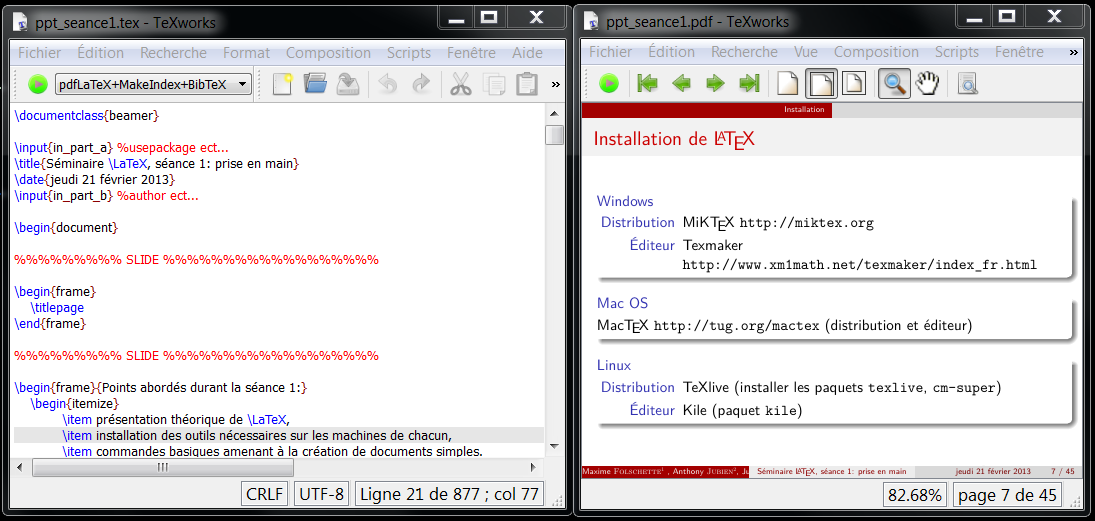
\includegraphics[width=11cm]{img/miktex_1}
\end{figure}

\end{frame}

%%%%%%%%% SLIDE %%%%%%%%%%%%%%%%%%

\begin{frame}{MacTeX (MacOS)}

\begin{figure}
\centering
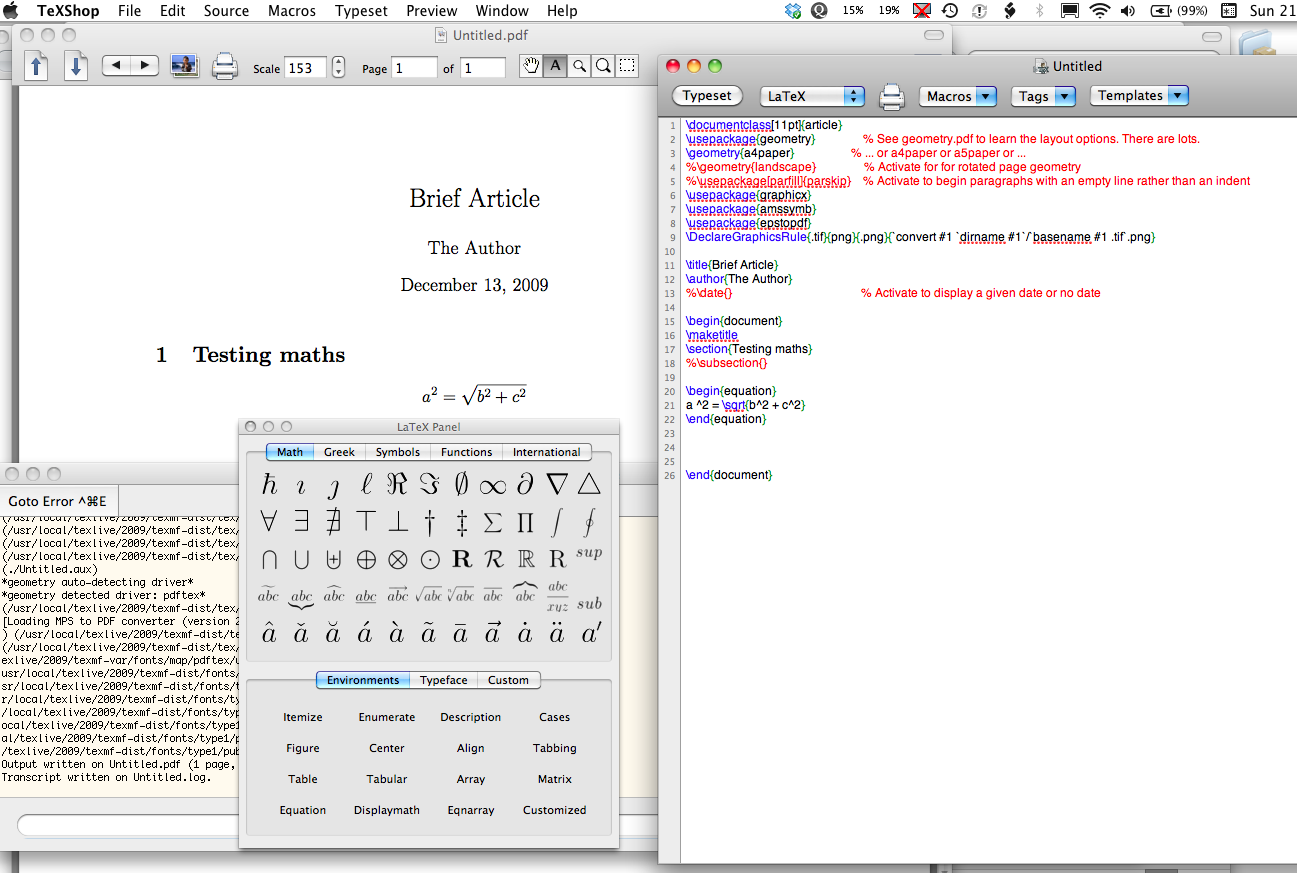
\includegraphics[width=9cm]{img/mactex_1}
\end{figure}

{\footnotesize image disponible sur http://trondlossius.no/articles/969-mactex-2009}

\end{frame}

%%%%%%%%% SLIDE %%%%%%%%%%%%%%%%%%

\begin{frame}{TeXlive (Linux)}

\begin{figure}
\centering
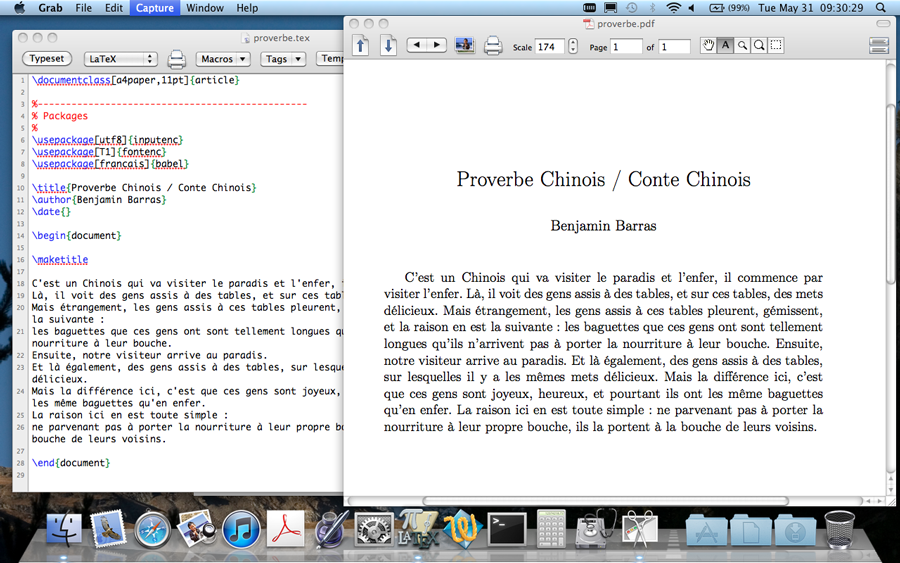
\includegraphics[width=10cm]{img/texlive_1}
\end{figure}

{\footnotesize image disponible sur http://flashinformatique.epfl.ch/spip.php?article2315}

\end{frame}


\section{Remarque} 

%%%%%%%%% SLIDE %%%%%%%%%%%%%%%%%%

\begin{frame}{Affichage}

2 fenêtres pour chaque distribution  \LaTeX
    \begin{itemize}
        \item fenêtre de gauche: éditeur \LaTeX (modification du .tex),
        \item fenêtre de droite: fichier .pdf généré.
    \end{itemize}


Intérêt ?
    \begin{itemize}
        \item Permet de voir le résultat généré instantanément, 
        \item permet de naviguer entre la source (.tex) et le fichier généré (.pdf) et vice-versa. 
    \end{itemize}

\end{frame}


%%%%%%%%% SLIDE %%%%%%%%%%%%%%%%%%

\section{Premier document}
\begin{frame}[fragile, label=firstdoc]{Premier document}
    \begin{lstlisting}[title={\texttt{minimal-*.tex}}]
        \documentclass[a4paper]{article}

        \usepackage[utf8]{inputenc}
        \usepackage[T1]{fontenc}
        \usepackage[french]{babel}

        \author{Preacutenom Nom}
        \title{Le titre}
        \date{\today}

        \begin{document}
            \maketitle
            Mon premier document
        \end{document}
    \end{lstlisting}
\end{frame}

%%%%%%%%% SLIDE %%%%%%%%%%%%%%%%%%

\begin{frame}{Compilation du premier document}
    \begin{enumerate}
        \item Ouvrir les documents \texttt{minimal-latin1.tex} et \texttt{minimal-utf8.tex};
        \item Fermer les documents présentant des accents bizarres;
        \item Compiler le document directement en pdf;
        \item Admirer le résultat!
    \end{enumerate}
\end{frame}

%%%%%%%%%%%%%%%%%%%%%%%%%%%%%%
%%%%%%%%%%%% PART %%%%%%%%%%%%%%%
%%%%%%%%%%%%%%%%%%%%%%%%%%%%%%

%\part{Introduction 2}

\section{Anatomie d'un document \LaTeX} 

%%%%%%%%% SLIDE %%%%%%%%%%%%%%%%%%

\begin{frame}[fragile, label=latex-struct]
    \frametitle{Structure de base d'un document \LaTeX}
    \begin{itemize}
        \item Classe du document \lstinline|\documentclass{classe}|
        \item Préambule
        \item Corps du document, entre \lstinline|\begin{document}| et \lstinline|\end{document}|
    \end{itemize}
\end{frame}

\againframe{firstdoc}


\section{Problèmes d'encodage} 

%%%%%%%%% SLIDE %%%%%%%%%%%%%%%%%%

\begin{frame}{Encodages}
    \begin{block}{Codage de caractères}
        Le codage de caractères est la transformation des caractères en octets.
        Il existe plusieurs codages, les plus connus étant:
        \begin{description}
            \item[ascii] Codage basé sur l'alphabet anglais.
            \item[ISO 8859-1] aussi appelé latin-1, codage reprenant le codage ascii, étendu aux langues européennes
            \item[utf-8] Codage standard regroupant un grand nombre de langues
        \end{description}
    \end{block}
\end{frame}

%%%%%%%%%%%%%%%%%%%%%%%%%%%%%%
%%%%%%%%%%%% PART %%%%%%%%%%%%%%%
%%%%%%%%%%%%%%%%%%%%%%%%%%%%%%

%\part{Rédiger un document scientifique} 

\section{Classes} 

%%%%%%%%% SLIDE %%%%%%%%%%%%%%%%%%

\begin{frame}[fragile]
    \frametitle{Des documents avec \texttt{class}}
    \begin{lstlisting}
        \documentclass[£\meta{option1}£, £\meta{option2}£]{£\meta{classe}£}
    \end{lstlisting}
    \begin{block}{Classes de document}
        \begin{itemize}
            \item \textbf{article} ou \textbf{proc}: pour les publications,
            \item \textbf{report}: pour les thèses et rapports,
            \item \textbf{beamer}: pour les présentation,
            \item \textbf{book}, \textbf{letter}, \dots : il y a du choix!
        \end{itemize}
    \end{block}
    \begin{block}{Options de classe}
        \begin{itemize}
            \item \textbf{Xpt} : changer la taille des caractères
            \item \textbf{a4paper}: marges pour l'impression en A4
            \item \textbf{twoside}: impression recto-verso
        \end{itemize}
    \end{block}
\end{frame}

%%%%%%%%% SLIDE %%%%%%%%%%%%%%%%%%

\begin{frame}[fragile]
    \frametitle{Classes \texttt{book} et \texttt{report}}
    \begin{block}{La classe \texttt{book}:}
        \begin{itemize}
 \item dispose d'une page de titre autonome, suivie d'une page blanche,
 \item peut se décomposer en parties, chapitres, sections, sous-sections, sous-sous-sections, paragraphes et sous-paragraphes.
 \item   Chaque partie et chapitre commence sur une page impaire,
   \item  les marges sont grandes pour faciliter la lecture.
        \end{itemize}
    \end{block}
    \begin{block}{La classe \texttt{report} est similaire à la classe  \texttt{book} sauf que:}
        \begin{itemize}
            \item  les chapitres ne commencent pas nécessairement en page impaire,
            \item dispose d'un environnement spécifique pour la mise en forme automatique d'un résumé.
        \end{itemize}
    \end{block}
\end{frame}

%%%%%%%%% SLIDE %%%%%%%%%%%%%%%%%%

\begin{frame}[fragile]
    \frametitle{Classe \texttt{article} et \texttt{proc}}
    \begin{block}{Comparé au classes \texttt{book} et \texttt{report} }
        \begin{itemize}
    \item  a son titre sur la même page que le début du texte,
     \item possède des marges étroites,
     \item ne peut pas contenir de chapitre.
        \end{itemize}
    \end{block}
\end{frame}



%%%%%%%%% SLIDE %%%%%%%%%%%%%%%%%%

\section{Paquets} 

\begin{frame}[fragile]
    \frametitle{ \texttt{Packages}}
        \begin{block}{Pourquoi? }
        \begin{itemize}
    \item les packages sont les bibliothèques utilisées pour des fonctions avancées,
     \item permet de palier un manque ou un besoin sous \LaTeX,
     \item beaucoup sont préinstallés avec votre distribution,
     \item ceux nécessaire seront téléchargés automatiquement. 
        \end{itemize}
    \end{block}

\end{frame}



%%%%%%%%% SLIDE %%%%%%%%%%%%%%%%%%

\section{Paquets} 

\begin{frame}[fragile]
    \frametitle{De nombreux \texttt{packages}}
    \begin{lstlisting}
        \usepackage[£\meta{option1}£, £\meta{option2}£]{£\meta{paquet}£}
    \end{lstlisting}
    \begin{block}{Paquets usuels}
        \begin{lstlisting}[multicols=2]
% accents
\usepackage[latin1]{inputenc}
\usepackage[T1]{fontenc}
%formules mathematiques
\usepackage{amsmath}
\usepackage{amsfonts}
\usepackage{amssymb}
%inclusion de fichier pdf
\usepackage{pdfpages}
%positionnement des figures
\usepackage{float}
%document en francais
\usepackage[francais]{babel}
%divers
\usepackage[left,pagewise]{lineno}
\usepackage{graphicx}
\usepackage{array}
        \end{lstlisting}
    \end{block}
\end{frame}


%%%%%%%%% SLIDE %%%%%%%%%%%%%%%%%%

\begin{frame}[fragile]
    \frametitle{Paquets \texttt{inputenc} et : \texttt{babel} }

    \begin{block}{Paquet \texttt{inputenc}  }
        \begin{itemize}
    \item  permet l'utilisation aisée des caratères accentués,
     \item est lié à une option d'encodage de caractères,
     \item Pour un documents en français: 
        \end{itemize}
\begin{lstlisting} 
\usepackage[latin1]{inputenc} 
\end{lstlisting}
    \end{block}

    \begin{block}{Paquet \texttt{babel}  }
        \begin{itemize}
    \item  permet de définir la langue du document,
     \item utilise pour la génération de l'index, table des matière...
     \item Pour un documents en français: 
        \end{itemize}
\begin{lstlisting} 
\usepackage[francais]{babel}
\end{lstlisting}
    \end{block}

\end{frame}

%%%%%%%%% SLIDE %%%%%%%%%%%%%%%%%%

\begin{frame}[fragile]
    \frametitle{Paquet \texttt{graphicx} :}

    \begin{block}{Le paquet \texttt{graphicx} :  }
        \begin{itemize}
    \item  permet l'utilisation de commandes spécifiques pour la gestion des figures (échelle taille, rotation, ect...),
     \item s'utilise avec la commande \texttt{ includegraphics}.
        \end{itemize}
    \end{block}


\end{frame}

%%%%%%%%% SLIDE %%%%%%%%%%%%%%%%%%

\begin{frame}[fragile]
    \frametitle{Paquets \texttt{amsfonts} et : \texttt{amsmath} }

    \begin{block}{Le paquet \texttt{amsfonts}  }
        \begin{itemize}
    \item  permet d’étendre les nombres de caractères compatibles avec la police par défaut de \LaTeX,
     \item utilisé pour les caractères mathématiques, les lettres en gras, etc...
        \end{itemize}
    \end{block}

    \begin{block}{Le paquet \texttt{amsmath}  }
        \begin{itemize}
    \item permet l’écriture des formules mathématiques,
     \item améliore la qualité typographique de leur rendu.
           \end{itemize}
    \end{block}

\end{frame}



%%%%%%%%% SLIDE %%%%%%%%%%%%%%%%%%

\begin{frame}[fragile]
\frametitle{Caractères spéciaux}

10 caractères spéciaux:
\begin{lstlisting}
\ $ & % # ^ _ { }
\end{lstlisting}

Ils peuvent être utilisés dans le texte:
\begin{lstlisting}
\textbackslash \$ \& \% \# \_ \{ \}
\end{lstlisting}

Les utilisés principales:
\begin{itemize}
\item\lstinline?%? indique que le restant de la ligne est en commentaire
\item\lstinline?$\dots$? indique une formule mathématique dans du texte
\item\lstinline?{\dots}? indique un groupe (groupe de caractères/mots)
\item\lstinline?\ \dots? indique le début d'une séquence de contrôle
\end{itemize}

\end{frame}

%%%%%%%%% SLIDE %%%%%%%%%%%%%%%%%%

\begin{frame}[fragile]
\frametitle{Chapitres, sections, sous-sections\dots}


Les commandes sont en début de chaque découpage
\begin{itemize}
\item\lstinline?\part{titre}?: partie
\item\lstinline?\chapter{titre}?: chapitre (uniquement pour les classes \texttt{report} et \texttt{book})
\item\lstinline?\section{titre}?: section
\item\lstinline?\subsection{titre}?: sous-section
\item\lstinline?\subsubsection{titre}?: sous-sous-section
\end{itemize}


Essayez d'utliser ces différentes commandes sous votre document \LaTeX  
 avec les classes  \texttt{article} et  \texttt{book} 

\end{frame}

%%%%%%%%%% SLIDE %%%%%%%%%%%%%%%%%%


\section{insertion}

\begin{frame}[fragile]
\frametitle{Commande d'insertion}

\begin{itemize}
\item\lstinline?\titlepage?: insère la page de titre
\item\lstinline?\clearpage?: insère un saut de page (1 maximum)
\item\lstinline?\newpage?: insère une nouvelle page
\item\lstinline?\cleardoublepage?: insère un saut de page sur page impaire
\item\lstinline?\tableofcontents?: insère une table des matières
\item\lstinline?\listoffigures?: insère une table des figures (séance 2)
\item\lstinline?\listoftables?: insère une table des tableaux (séance 2)
\item \dots
\end{itemize}

Essayez d'utliser les commandes   \texttt{titlepage}  \texttt{clearpage}  et \texttt{tableofcontents}  sous votre document \LaTeX 

\end{frame}


%%%%%%%%% SLIDE %%%%%%%%%%%%%%%%%%
\section{Paragraphe}

\begin{frame}[fragile]
\frametitle{Quelques règles}

\begin{itemize}
\item un saut de paragraphe est produit par une ligne vierge
\item\LaTeX{} ignore les sauts de ligne et les espaces multiples (mise en forme automatique à la compilation)
\end{itemize}

% Note : Les « £\`e£ » permettent de mettre des accents dans les listings
\begin{lstlisting}
| Premier paragraphe.
| 
| Deuxi£\`e£me paragraphe apr£\`e£s deux sauts de ligne.
| 
| 
| Dernier      paragraphe    plus      loin.
\end{lstlisting}

donne:

\medskip
Premier paragraphe.

Deuxième paragraphe après deux sauts de ligne.


Dernier      paragraphe    plus      loin.

\medskip

Regardez sur votre document \LaTeX{} l'effet des sauts de ligne...

\end{frame}

%%%%%%%%% SLIDE %%%%%%%%%%%%%%%%%%

\begin{frame}[fragile]
\frametitle{Taille et style des caractères}

Différentes tailles et styles de caractères sont possibles:
\begin{lstlisting}
\tiny, \scriptsize, \footnotesize, \small, \normalsize,
\large, \Large, \LARGE, \huge, \Huge
\end{lstlisting}

\tiny Aze \normalsize \scriptsize Aze \normalsize \footnotesize Aze \normalsize \small Aze \normalsize \normalsize Aze \normalsize

\large Aze \normalsize\Large Aze \normalsize\LARGE Aze \normalsize \huge Aze \normalsize \Huge Aze \normalsize

\begin{lstlisting}
\textbf{gras} \textit{italique} \textsc{majuscules}
\end{lstlisting}

\textbf{Aze } \textit{Aze } \textsc{Aze }

Regardez sur votre document \LaTeX   l'effet des différentes tailles et styles de caractères.

\end{frame}



%%%%%%%%% SLIDE %%%%%%%%%%%%%%%%%%

\section{Environnement}

\begin{frame}[fragile]
\frametitle{Environnement}

\begin{lstlisting}
\begin{nom-environnement}
...
...    % Contenu de l'environnement
...
\end{nom-environnement}
\end{lstlisting}

Permet de définir le début de la fin d'un environnement (figures, équations mathématiques, ect\dots)
\end{frame}

%%%%%%%%% SLIDE %%%%%%%%%%%%%%%%%%


%
%%%%%%%%%%%
%\begin{frame}[fragile]
%\frametitle{Environnement figure}
%
%\begin{lstlisting}
%\begin{figure} %debut de l'environnement figure
%\centering %figure centree
%\includegraphics[width=Xcm]{nom_image} % image de X cm de large
%\caption{Titre de la figure} %titre de la figure
%\label{titre_fig} %label de la figure (ex voir figure W)
%\end{figure} %fin de l'environnement figure
%\end{lstlisting}
%
%Permet d'insérer une image (format: jpg, gif, pdf\dots.), inutile de préciser l'extension du fichier
%
%\vspace{5mm}
%
%\lstinline?\begin{figure}? : figure en objet flottant (\LaTeX gère la mise en page)
%
%\vspace{5mm}
%
%\lstinline?\begin{figure}[h]? : affiche la figure à l'endroit voulu (déconseillé)
%
%\vspace{5mm}
%
%On pourra faire référence à la figure avec \lstinline?\ref{titre_fig}?
%
%\end{frame}
%
%%%%%%%%%% SLIDE %%%%%%%%%%%%%%%%%%
%
%\begin{frame}[fragile]
%\frametitle{Environnement équation}
%
%\begin{lstlisting}
%\begin{equation} %debut de l'environnement equation
%1+1=0 %equation
%\label{titre_eq} %label de l'equation (ex voir equation W)
%\end{equation} %fin de l'environnement equation
%\end{lstlisting}
%
%Permet d'insérer une équation mathématique
%\end{frame}
%
%%%%%%%%%% SLIDE %%%%%%%%%%%%%%%%%%
%
%\begin{frame}[fragile]
%\frametitle{Environnement itemize}
%
%
%\begin{lstlisting}
%\begin{itemize} %debut de l'environnement itemize
%\item texte 1 %item 1
%\item texte 2 %item 2
%\end{itemize} %fin de l'environnement itemize
%\end{lstlisting}
%
%
%Permet d'insérer une liste à puces
%\end{frame}
%
%%%%%%%%%% SLIDE %%%%%%%%%%%%%%%%%%
%
%\begin{frame}[fragile]
%\frametitle{Autres commandes}
%
%\begin{itemize}
%\item\lstinline?\titlepage?: insère la page de titre
%\item\lstinline?\clearpage?: insère un saut de page
%\item\lstinline?\tableofcontents?: insère une table des matières
%\item\lstinline?\listoffigures?: insère une table des figures
%\item\lstinline?\listoftables?: insère une table des tableaux
%\item \dots
%\end{itemize}
%
%\end{frame}
%
%%%%%%%%%% SLIDE %%%%%%%%%%%%%%%%%%
%
%\begin{frame}
%\frametitle{Fin de la première partie}
%
%\LARGE
%Fin de la première partie
%\normalsize \color{black}
%
%\end{frame}
%% }}}
%
%
%
%\section{Équations mathématiques}
%
%%%%%%%%%% SLIDE %%%%%%%%%%%%%%%%%%
%
%\begin{frame}[fragile]
%\frametitle{Mathématiques sous LaTeX}
%
%\begin{itemize}
%\item \sout{éditeur d'équation nécessaire}
%\item\sout{souris}
%\item nécessité de connaitre les commandes usuelles
%\item possibilité d'insérer des équation dans du texte: blabla $1+1=4$ blabla
%\item possibilité d'insérer des équations entre deux paragraphes et de les numéroter automatiquement:
%\end{itemize}
%
%\begin{equation}
%1+1=4
%\end{equation}
%
%\end{frame}
%
%%%%%%%%%% SLIDE %%%%%%%%%%%%%%%%%%
%
%\begin{frame}[fragile]
%\frametitle{équation ou notation mathématique dans le texte}
%
%\begin{lstlisting}
%blabla $\pi$ blabla $1+1=0$ blabla
%\end{lstlisting}
%
%donne:
%
%\vspace{5mm}
%
%blabla $\pi$ blabla $1+1=0$ blabla
%
%\end{frame}
%
%%%%%%%%%% SLIDE %%%%%%%%%%%%%%%%%%
%
%\begin{frame}[fragile]
%\frametitle{Environnement équation }
%
%\begin{lstlisting}
%\begin{equation} %debut de l'environnement equation
%1+1=0 %equation
%\label{titre_eq} %label de l'equation (ex voir equation W)
%\end{equation} %fin de l'environnement equation
%\end{lstlisting}
%
%donne:
%
%\begin{equation} %début de l'environnement équation
%1+1=0 %équation
%\label{titre_éq} %label de l'équation (ex voir équation W)
%\end{equation} %fin de l'environnement équation
%
%\end{frame}
%
%%%%%%%%%% SLIDE %%%%%%%%%%%%%%%%%%
%
%\begin{frame}[fragile]
%\frametitle{Commandes usuelles 1}
%
%\begin{itemize}
%\item\lstinline?\sqrt{1+1}?: racine carrée $\Longrightarrow \sqrt{1+1}$
%\item\lstinline?\sqrt[2]{1+1}?: racine carrée n-ième $ \Longrightarrow \sqrt[3]{1+1}$
%\item\lstinline?\frac{1}{2}?: fraction $\Longrightarrow \frac{1}{2}$
%\item\lstinline?\sin (1+1)?: cosinus $\Longrightarrow\sin (1+1)$
%\item\lstinline?\cos (1+1)?: sinus $\Longrightarrow \cos (1+1)$
%\item\lstinline?1^{1+1} ou 1^1?: puissance $\Longrightarrow 1^{1+1}$ ou $1^1$
%\item\lstinline?1_{1+1} ou 1_1?: indice $\Longrightarrow1_{1+1}$ ou $1_1$
%\item\lstinline?1_{1+1}^{1+1} ou 1_1^1?: puissance ET indice $\Longrightarrow 1_{1+1}^{1+1}$ ou $1_1^1$
%\end{itemize}
%\end{frame}
%
%%%%%%%%%% SLIDE %%%%%%%%%%%%%%%%%%
%
%\begin{frame}[fragile]
%\frametitle{Commandes usuelles 2}
%
%\begin{itemize}
%\item \lstinline? \begin{pmatrix} 1 & 2 \\ 3 & 4 \end{pmatrix}?: matrice type 'p' $ \begin{pmatrix} 1 & 2 \\ 3 & 4 \end{pmatrix}$
%\item \lstinline? \begin{bmatrix} 1 & 2 \\ 3 & 4 \end{bmatrix}?: matrice type 'b' $ \begin{bmatrix} 1 & 2 \\ 3 & 4 \end{bmatrix}$
%\item \lstinline? \begin{Bmatrix} 1 & 2 \\ 3 & 4 \end{Bmatrix}?: matrice type 'B' $ \begin{Bmatrix} 1 & 2 \\ 3 & 4 \end{Bmatrix}$
%\item \lstinline? \begin{vmatrix} 1 & 2 \\ 3 & 4 \end{vmatrix}?: matrice type 'v' $ \begin{vmatrix} 1 & 2 \\ 3 & 4 \end{vmatrix}$
%\item \lstinline? \begin{Vmatrix} 1 & 2 \\ 3 & 4 \end{Vmatrix}?: matrice type 'V' $ \begin{Vmatrix} 1 & 2 \\ 3 & 4 \end{Vmatrix}$
%\end{itemize}
%
%
%\end{frame}
%
%%%%%%%%%%%
%\begin{frame}[fragile]
%\frametitle{Commandes usuelles 3}
%
%\begin{itemize}
%\item \lstinline? \dot{v} \ddot{v} \dddot{v} \ddddot{v}?: dérivée $ \dot{v}$ $\ddot{v}$ $\dddot{v}$ $\ddddot{v}$
%\item \lstinline? \vec{AB}?: vecteur $\vec{AB}$
%\item \lstinline? \overline{1+i}?: conjugué $ \overline{1+i} $
%\item \lstinline? \sum_a^b ?: somme $ \sum_a^b $
%\item \lstinline? \int_a^b ?: intégrale $ \int_a^b $
%\item \lstinline? \widehat {ABC}?: angle $ \widehat {ABC}$
%\item \lstinline? 1+1 \mbox{ idem que } 1+1?: texte $ 1+1 \mbox{ idem que } 1+1$
%\item \lstinline? \left( \frac{1}{2} \right) ?: parenthèse $ \left( \frac{1}{2} \right)$
%\end{itemize}
%
%\end{frame}
%
%%%%%%%%%%%
%\begin{frame}[fragile]
%\frametitle{Caractère grec}
%
%\begin{itemize}
%\item idée: nom de la lettre grec ( Nom : Lettre majuscule; nom: lettre minuscule)
%\end{itemize}
%
%Exemples:
%
%\lstinline?\Lambda?: donne $\Lambda$
%
%\lstinline?\lambda?: donne $\lambda$
%\end{frame}
%
%
%%%%%%%%%%%
%\begin{frame}[fragile]
%\frametitle{Example d'équation complexe}
%
%\begin{lstlisting}
%A= \left(
%\sqrt{\sum_{k=0}^{1000} \overline{5 k+i} }
%\begin{bmatrix}
%1 & 2 & a \\
%3 & 4 & b \\
%5 & 6 & c \\
%7 & 8 & d
%\end{bmatrix}
%\frac{1+3+9+o+\frac{1}{2}} {n-m-\lambda}
%\right)
%\end{lstlisting}
%
%donne:
%\begin{equation} %début de l'environnement équation
%A= \left(
%\sqrt{\sum_{k=0}^{1000} \overline{5 k+i} }
%\begin{bmatrix} 1 & 2 & a \\ 3 & 4 & b \\ 5 & 6 & c \\ 7 & 8 & d\end{bmatrix}
%\frac{1+3+9+o+\frac{1}{2}} {n-m-\lambda}
%\right)
%\label{titre_éq} %label de l'équation (ex voir équation W)
%\end{equation} %fin de l'environnement équation
%\end{frame}
%
%%%%%%%%%%%
%\begin{frame}[fragile]
%\frametitle{Fin de la deuxième partie}
%
%\LARGE
%Fin de la deuxième partie
%\normalsize
%
%\end{frame}
%
%%%%%%%%%%%%%%%%%%%%%%%%%%%%%%%%%%%%%%%%%%%%%%
%%%%%%%%%PARTIE 3
%%%%%%%%%%%%%%%%%%%%%%%%%%%%%%%%%%%%%%%%%%%%%
%
%%%%%%%%%%%
%
%\section{Tableaux}
%
%%%%%%%%%%%
%\begin{frame}[fragile]
%\frametitle{Tableau sous LaTeX}
%
%\begin{itemize}
%\item assez rébarbatif (point faible de \LaTeX)
%\item nécessité d'être TRES rigoureux
%\end{itemize}
%
%\end{frame}
%
%
%
%%%%%%%%%%%
%\begin{frame}[fragile]
%\frametitle{Environnement tabular}
%
%\begin{lstlisting}
%\begin{table} %debut de l'environnement table
%\centering %tableau centre
%\begin{tabular}{|l|c|r|}%debut de l'environnement tabular
%\hline %ligne
%colonne 1 & colonne 2 & colonne 3 \\
%\hline %ligne
%1 & 1 & 3 \\
%2 & 2 & 4 \\
%\hline %ligne
%\end{tabular} %fin de l'environnement tabular
%\label{titre_tab} %label de du tableau (ex voir tableau W)
%\end{table} %fin de l'environnement table
%\end{lstlisting}
%
%donne:
%
%\begin{table} %début de l'environnement table
%\centering %tableau centré
%\begin{tabular}{|l|c|r|}%début de l'environnement tabular
%\hline
%colonne 1 & colonne 2 & colonne 3 \\
%\hline
%1 & 1 & 3 \\
%2 & 2 & 4 \\
%\hline
%\end{tabular}
%\label{titre_tab} %label de du tableau (ex voir tableau W)
%\end{table}
%
%\end{frame}
%
%
%%%%%%%%%%%
%\begin{frame}[fragile]
%\frametitle{Base pour un tableau}
%
%\begin{itemize}
%\item une ligne horizontale apparait avec \lstinline?\hline?
%\item la déclaration des colonnes s'effectue au début dans la deuxième paire d'accolade \lstinline?\begin{tabular}{|l|c|r|}?
%\end{itemize}
%
%Avec:
%
%\begin{itemize}
%\item \lstinline?l? pour une colonne alignée à gauche
%\item \lstinline?r? pour une colonne alignée à droite
%\item \lstinline?c? pour une colonne centrée
%\item \lstinline?|? pour un trait vertical entre chaque colonne (Alt Gr + 6 )
%\item \lstinline?||? pour un double trait vertical entre chaque colonne
%\end{itemize}
%
%\end{frame}
%
%
%%%%%%%%%%%
%\begin{frame}[fragile]
%\frametitle{Fusion ligne/colonne}
%
%\begin{itemize}
%\item Fusion de nb colonnes \lstinline?\multicolumn{nb}{c|c|}{texte}?
%\item Fusion de lignes entre excluant les colonnes nb1 et nb2 \lstinline?\cline{nb1-nb2} ?
%\end{itemize}
%
%
%\end{frame}
%
%%%%%%%%%%%
%\begin{frame}[fragile]
%\frametitle{Exemple de fusion de colonnes}
%
%\begin{lstlisting}
%[\dots]
%\begin{tabular}{|l|c|r|}%debut de l'environnement tabular
%\hline %ligne
%colonne 1 & colonne 2 & colonne 3 \\
%\hline %ligne
%1 & \multicolumn{2}{c|}{13} \\
%\hline
%2 & 2 & 4 \\
%\hline %ligne
%\end{tabular} %fin de l'environnement tabular
%[\dots]
%\end{lstlisting}
%
%donne:
%
%\begin{table} %début de l'environnement table
%\centering %tableau centré
%\begin{tabular}{|l|c|r|}%début de l'environnement tabular
%\hline
%colonne 1 & colonne 2 & colonne 3 \\
%\hline
%\hline %ligne
%1 & \multicolumn{2}{c|}{13} \\
%\hline
%2 & 2 & 4 \\
%\hline
%\end{tabular}
%\label{titre_tab} %label de du tableau (ex voir tableau W)
%\end{table}
%
%\end{frame}
%
%%%%%%%%%%%
%\begin{frame}[fragile]
%\frametitle{Exemple de fusion de lignes}
%
%\begin{lstlisting}
%[\dots]
%\begin{tabular}{|l|c|r|}%debut de l'environnement tabular
%\hline %ligne
%colonne 1 & colonne 2 & colonne 3 \\
%\hline %ligne
%1 & 1 & 3 \\
%\cline{2-3}
%& 2 & 4 \\
%\hline %ligne
%\end{tabular} %fin de l'environnement tabular
%[\dots]
%\end{lstlisting}
%
%donne:
%
%\begin{table} %début de l'environnement table
%\centering %tableau centré
%\begin{tabular}{|l|c|r|}%début de l'environnement tabular
%\hline %ligne
%colonne 1 & colonne 2 & colonne 3 \\
%\hline %ligne
%1 & 1 & 3 \\
%\cline{2-3}
%& 2 & 4 \\
%\hline %ligne
%\end{tabular}
%\label{titre_tab} %label de du tableau (ex voir tableau W)
%\end{table}
%
%\end{frame}
%
%
%%%%%%%%%%%
%\begin{frame}[fragile]
%\frametitle{Fin de la troisième partie}
%
%\LARGE
%Fin de la troisième partie
%\normalsize
%
%\end{frame}
%
%%%%%%%%%%%%%%%%%%%%%%%%%%%%%%%%%%%%%%%%%%%%%%
%%%%%%%%%PARTIE 3
%%%%%%%%%%%%%%%%%%%%%%%%%%%%%%%%%%%%%%%%%%%%%
%
%%%%%%%%%%%
%
%\section{Bibliographie avec BibTeX}
%
%%%%%%%%%%%
%
%\begin{frame}[fragile]
%\frametitle{Présentation de BibTeX}
%BibTeX est un outil de gestion de bibliographie
%	
%
%La \emph{base de données} bibliographique est placée dans un fichier extérieur (.bib)
%On le place dans le document par
%\begin{lstlisting}
%\bibliographystyle{plain}
%\bibliography{nom-biblio}
%\end{lstlisting}
%On y fait référence par la commande \lstinline?\cite{\dots}?\cite{latexcompanion}
%
%Il est possible d'inclure plusieurs fichiers biblio:
%\lstinline?\bibliography{biblio1,biblio2}?
%\end{frame}
%
%\begin{frame}
%\frametitle{Styles de bibliographie}
%Les styles biblioraphiques (.bst) sont généralement fournis par le journal ou la revue.
%
%Sinon, il est possible d'utiliser les styles \emph{abbrv-fr}, \emph{alpha-fr}
%\end{frame}
%
%\begin{frame}[fragile]
%\frametitle{Ajout de nouvelles entrées}
%
%Large choix de type d'entrée: article, book, booklet, inproceedings, manual, pdhthesis, techreport, unpublished, misc.
%
%
%Exemple:
%\begin{lstlisting}
%@book{goossens93,
%author = "Goossens, Michel and Mittlebach, Frank",
%title = "The Latex Companion",
%year = "1993",
%publisher = "Addison-Wesley",
%address = "Reading, Massachusetts"
%}
%\end{lstlisting}
%\end{frame}
%
%
%\begin{frame}
%\frametitle{Outils de gestion de bibliographie}
%
%La plupart des bases de données bibliographiques permettent d'exporter une entrée en BibTeX.
%
%Dans le cas contraire, utiliser un outil de gestion de bibliographie:
%\begin{itemize}
%\item Mendeley;
%\item JabRef;
%\item \dots
%\end{itemize}
%\end{frame}
%
%\begin{frame}
%\frametitle{Bibliographie}
%\nocite{*} % Bad, should change
%\bibliographystyle{abbrv-fr}
%\bibliography{latex}
%\end{frame}



%%%%%%%%%%%%%%%%%%%%%%%%%%%%%%%%%%%%%%%%%%%%%%%%%%%%%%%%%%%%%%%%%%%%%%%%%%%%%%%%%%
%%%%%%%%%%%%%%%%%%%%%%%% FIN DU DOCUMENT %%%%%%%%%%%%%%%%%%%%%%%%%%%%%%%%%%%%%%%%%%%%%%%%
%%%%%%%%%%%%%%%%%%% ( NON PRISE EN COMPTE DE LA SUITE ) %%%%%%%%%%%%%%%%%%%%%%%%%%%%%%%%%%%%%%%%%%%
\end{document}
%%%%%%%%%%%%%%%%%%%%%%%%%%%%%%%%%%%%%%%%%%%%%%%%%%%%%%%%%%%%%%%%%%%%%%%%%%%%%%%%%%
%%%%%%%%%%%%%%%%%%%%%%%%%%%%%%%%%%%%%%%%%%%%%%%%%%%%%%%%%%%%%%%%%%%%%%%%%%%%%%%%%%
